\chapter{Results \& Analysis}
\label{sec:results}

\section{Main classification results}

Table~\ref{tab:mainresults} reports macro-F1 and Ia-vs-rest ROC-AUC for
every trained configuration, alongside a majority-class and a five-feature
logistic-regression baseline fit on each tier with the frozen evaluation
harness. Every Tier B number is measured on zeropoint-corrected photometry
(Section~\ref{sec:silentfailures}); fine-tuned Tier B rows are the mean over
\TierBNSeeds{} seeds with identical data and object order, so a difference
between configurations can be read against the seed-to-seed spread.

\begin{table}[htb]
\centering
\caption{Main classification results at the full light-curve cutoff.
Per-class F1 columns are Ia/Ib-c/II in order. Fine-tuned Tier B rows are
the mean over \TierBNSeeds{} seeds, with the standard deviation of
macro-F1 in parentheses; zero-shot rows are inference-only and
seed-independent. The deployed configuration is marked; its served
checkpoint is the seed-42 run (macro-F1 \DeployedMacroF{}, Ia-vs-rest
ROC-AUC \DeployedRocAucIa{}, Ib/c F1 \DeployedFIbc{}). Output probabilities
carry the training-set class prior, not the real sky prior
(Section~\ref{sec:discussion}).}
\label{tab:mainresults}
\small
\begin{tabular}{L{4.6cm}rrrrr}
\toprule
Configuration & Macro-F1 & ROC-AUC (Ia) & F1 Ia & F1 Ib/c & F1 II \\
\midrule
Tier A, majority class & \BaselineMajTierAMacroF{} & \BaselineMajTierARocAucIa{} &
  \BaselineMajTierAFIa{} & \BaselineMajTierAFIbc{} & \BaselineMajTierAFII{} \\
Tier A, logistic regression & \BaselineLRTierAMacroF{} & \BaselineLRTierARocAucIa{} &
  \BaselineLRTierAFIa{} & \BaselineLRTierAFIbc{} & \BaselineLRTierAFII{} \\
Tier A, LC-only & \TierLCOnlyMacroFFull{} & \TierLCOnlyRocAucIaFull{} &
  \TierLCOnlyFIaFull{} & \TierLCOnlyFIbcFull{} & \TierLCOnlyFIIFull{} \\
Tier A, LC+static & \TierLCStaticMacroFFull{} & \TierLCStaticRocAucIaFull{} &
  \TierLCStaticFIaFull{} & \TierLCStaticFIbcFull{} & \TierLCStaticFIIFull{} \\
Tier A, LC+static, no photo-$z$ & \TierLCStaticNoPhotozMacroFFull{} &
  \TierLCStaticNoPhotozRocAucIaFull{} & \TierLCStaticNoPhotozFIaFull{} &
  \TierLCStaticNoPhotozFIbcFull{} & \TierLCStaticNoPhotozFIIFull{} \\
Tier A, WHXE head & \TierWHXEMacroFFull{} & \TierWHXERocAucIaFull{} &
  \TierWHXEFIaFull{} & \TierWHXEFIbcFull{} & \TierWHXEFIIFull{} \\
\midrule
Tier B, majority class & \BaselineMajTierBMacroF{} & \BaselineMajTierBRocAucIa{} &
  \BaselineMajTierBFIa{} & \BaselineMajTierBFIbc{} & \BaselineMajTierBFII{} \\
Tier B, logistic regression & \BaselineLRTierBMacroF{} & \BaselineLRTierBRocAucIa{} &
  \BaselineLRTierBFIa{} & \BaselineLRTierBFIbc{} & \BaselineLRTierBFII{} \\
Tier B, zero-shot, LC-only weights & \ZeroShotLCOnlyMacroF{} &
  \ZeroShotLCOnlyRocAucIa{} & \ZeroShotLCOnlyFIa{} & \ZeroShotLCOnlyFIbc{} &
  \ZeroShotLCOnlyFII{} \\
Tier B, zero-shot, LC+static weights & \ZeroShotMacroF{} &
  \ZeroShotRocAucIa{} & \ZeroShotFIa{} & \ZeroShotFIbc{} & \ZeroShotFII{} \\
Tier B, LC-only fine-tune & \LCOnlyMacroF{} (\LCOnlyMacroFSD{}) &
  \LCOnlyRocAucIa{} & \LCOnlyFIa{} & \LCOnlyFIbc{} & \LCOnlyFII{} \\
Tier B, LC+static fine-tune \textbf{(deployed)} & \WithStaticMacroF{}
  (\WithStaticMacroFSD{}) & \WithStaticRocAucIa{} & \WithStaticFIa{} &
  \WithStaticFIbc{} & \WithStaticFII{} \\
Tier B, LC+static+DRB fine-tune & \WithStaticDRBMacroF{}
  (\WithStaticDRBMacroFSD{}) & \WithStaticDRBRocAucIa{} & \WithStaticDRBFIa{} &
  \WithStaticDRBFIbc{} & \WithStaticDRBFII{} \\
\bottomrule
\end{tabular}
\end{table}

The sim-to-real gap is measured between matched configurations, so that it
isolates the change of data rather than a change of model. For the
deployed LC+static configuration it is
$\TierLCStaticMacroFFull{} \to \WithStaticMacroF{}$, a drop of
$\SimToRealGapStatic{}$ macro-F1; for LC-only it is
$\TierLCOnlyMacroFFull{} \to \LCOnlyMacroF{}$, a drop of
$\SimToRealGapLCOnly{}$. Both are the expected direction: simulated data has
no instrument noise, no real-bogus artifacts, and no mislabelled hosts, so
it is strictly easier than reality, and a model that scored identically on
both would be the stronger signal of a broken (leaking) evaluation split,
not of a better model. Fine-tuning recovers $\TransferGain{}$ macro-F1 over
the matching zero-shot model for LC+static
($\ZeroShotMacroF{} \to \WithStaticMacroF{}$) and $\TransferGainLCOnly{}$ for
LC-only ($\ZeroShotLCOnlyMacroF{} \to \LCOnlyMacroF{}$) -- fine-tuning is
doing real, measurable work, not re-labelling an already-adequate zero-shot
model. Host features help on both tiers: by $\PhotozGainWith{}$ macro-F1 on
Tier A and by $\StaticGainTierB{}$ on Tier B, \StaticGainOverSD{} times the larger of
the two configurations' seed-to-seed standard deviations, which is why
LC+static is the deployed configuration.

\section{Phase curve}

\begin{figure}[htb]
\centering
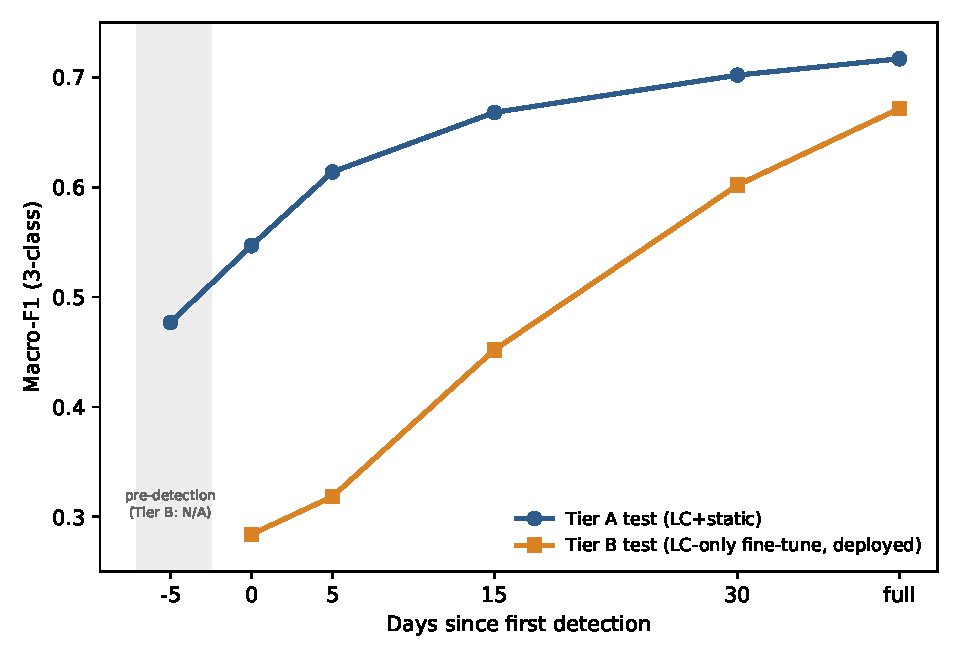
\includegraphics[width=0.78\linewidth]{figures/fig4_phase_curve}
\caption{Macro-F1 as a function of days since first detection, Tier A test
(LC+static) against Tier B test (LC+static fine-tune, the deployed
checkpoint; every point, including the full cutoff, read from that one
run's own evaluation). Tier B has no pre-detection ($-5$\,d) point because
its source metadata contains no forced-photometry row type at all
(Section~\ref{sec:discussion}); the comparison is therefore restricted to
cutoffs $\geq 0$. Conflating ``the model degrades on real data'' with ``the
model was evaluated on an easier phase slice'' would compare a full Tier A
curve (which includes $-5$\,d) against a necessarily truncated Tier B one
and misstate the size of the sim-to-real gap for reasons that have nothing
to do with sim-to-real generalisation.}
\label{fig:phasecurve}
\end{figure}

Both curves in Figure~\ref{fig:phasecurve} rise monotonically with more of
the light curve observed, from \TierLCStaticMacroFZero{} (Tier A, $0$\,d) to
\TierLCStaticMacroFFull{} (full) and from \DeployedPhaseZero{} (Tier B, $0$\,d)
to \DeployedPhaseFull{} (full). A model that got \emph{worse} with more data
would itself indicate a bug -- leakage that only helps a truncated input,
or an architecture unable to use a long sequence -- so the monotonic shape
is a sanity check that passed, not merely a pleasant picture.

\section{Confusion matrices}

\begin{figure}[htb]
\centering
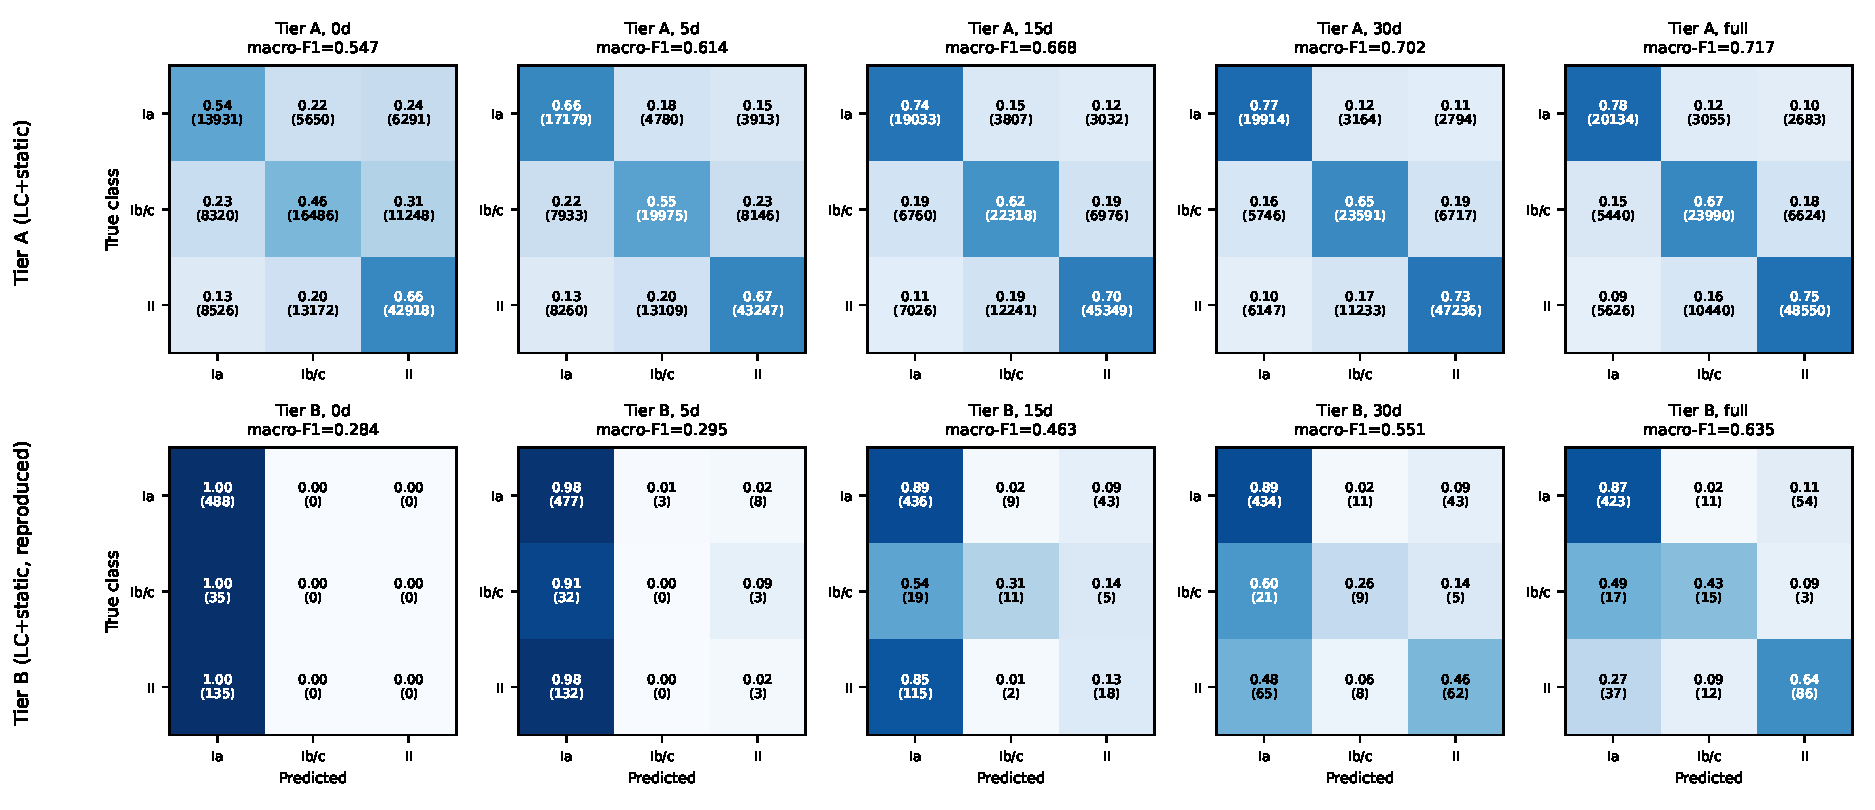
\includegraphics[width=\linewidth]{figures/fig5_confusion_grid}
\caption{Row-normalised confusion matrices (raw counts in parentheses) at
each phase cutoff. Top row: Tier A test, LC+static. Bottom row: Tier B
test, the deployed LC+static fine-tune (seed 42), read from that run's own
evaluation. At the earliest cutoffs the Tier B model predicts Ia for
\DeployedPhaseZeroPredIaFrac{}\% of objects at $0$\,d, the majority class;
the diagonal emerges as photometry accumulates.}
\label{fig:confgrid}
\end{figure}

\section{Prediction panels}

\begin{figure}[htb]
\centering
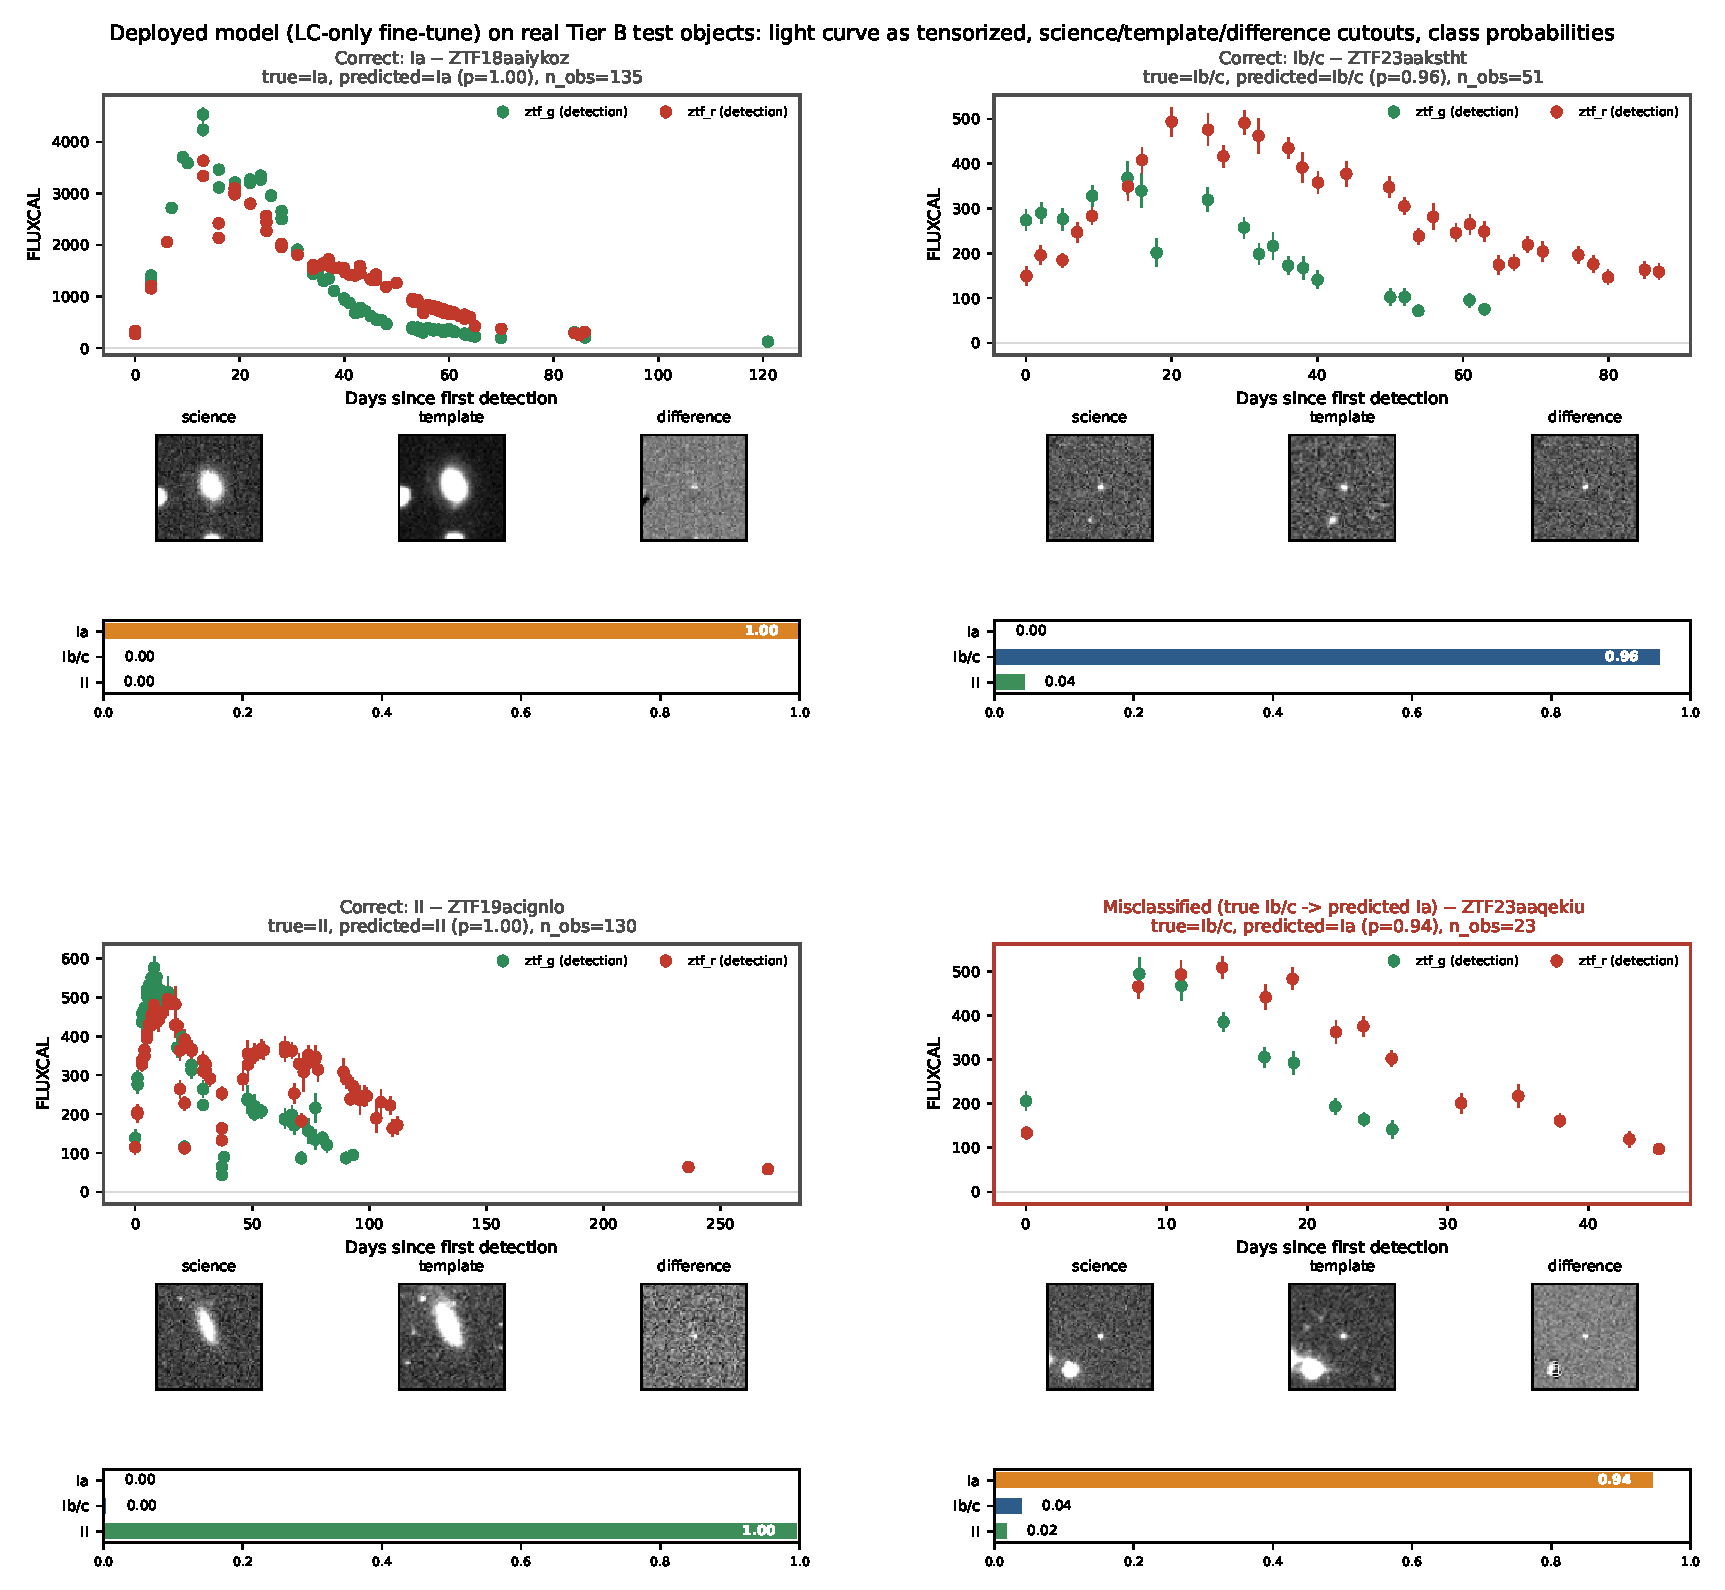
\includegraphics[width=0.92\linewidth]{figures/fig6_prediction_panels}
\caption{Four real Tier B test-split objects, run through the deployed
checkpoint (LC+static fine-tune) at inference time: the light curve as
tensorized (detections filled, forced photometry as small crosses, ZTF
$g$/$r$ in distinct colours), the real science/template/difference cutout
triplet (ZScale-rendered), and the model's own class-probability bars.
\emph{Selection}: for each class, the highest-confidence correctly
classified test object with at least \PanelMinObs{} observations (falling back to the
best available if no such object exists for a class); for the
misclassification panel, among test objects truly Ib/c but predicted Ia --
this project's own recorded dominant confusion -- the most confident wrong
call, tie-broken toward the sparser light curve. All four objects shown
were found by this selection rule on the first pass; none were
cherry-picked from a larger, unreported set of alternatives.}
\label{fig:predpanels}
\end{figure}

The misclassified panel in Figure~\ref{fig:predpanels} is instructive on
its own: a \PanelMisclassNObs{}-observation light curve is called Ia at
\PanelMisclassConfidencePct{}\% confidence while its spectroscopic type is
Ib/c -- exactly the kind of case the Ib/c F1 figure in
Table~\ref{tab:mainresults} summarises as a single number.

\section{Anomaly branch under domain shift}

\begin{figure}[htb]
\centering
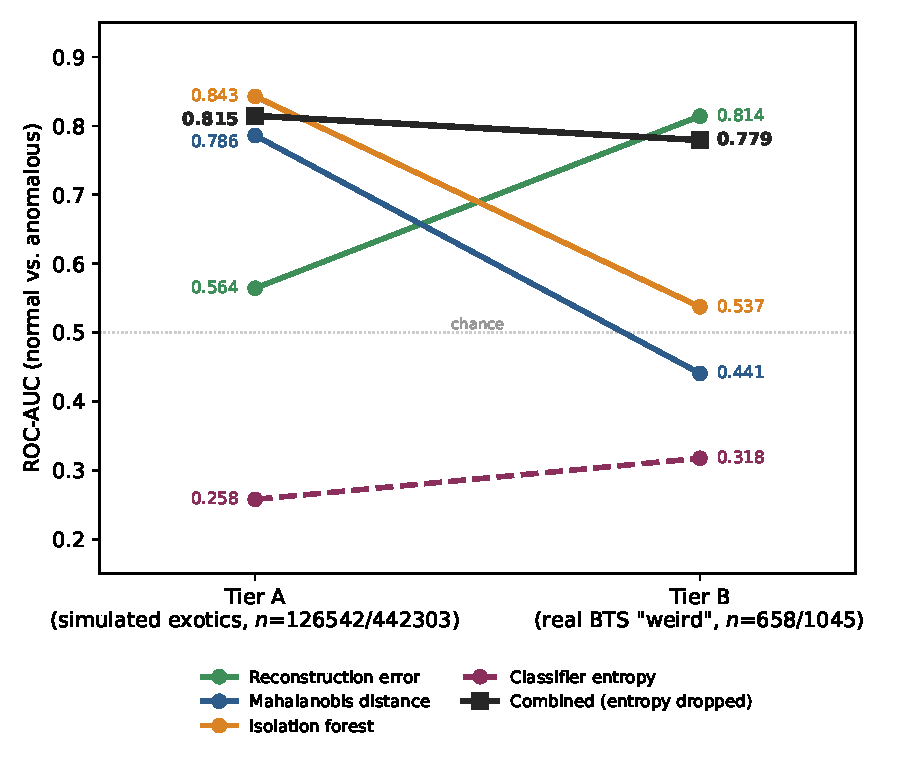
\includegraphics[width=0.62\linewidth]{figures/fig7_anomaly_slope}
\caption{Each anomaly-score component's normal-vs-anomalous ROC-AUC, Tier A
(simulated exotic classes held out of classifier training) against Tier B
(real, spectroscopically confirmed non-supernova BTS objects). The two
latent-space methods (isolation forest, Mahalanobis distance) fall toward
chance under the sim-to-real domain shift; reconstruction error rises. The
combined score (entropy dropped, black) is not the best score on either
individual set -- isolation forest alone beats it on Tier A, reconstruction
error alone beats it on Tier B -- but it is the only score that stays
useful on \emph{both}.}
\label{fig:anomalyslope}
\end{figure}

Table~\ref{tab:anomaly} gives the same comparison numerically, including
the combination with and without classifier entropy. Entropy was tested as
a fourth component and dropped: rather than being merely unhelpful, it was
actively \emph{harmful} to the combination on both evaluation sets, and its
own behaviour is the more interesting finding
(Section~\ref{sec:discussion}) -- it is markedly \emph{more} confident
(mean entropy \EntropyTierAExotic{} on Tier A's held-out exotic classes
versus \EntropyTierANormal{} on Tier A's own in-distribution test set; the
same direction, \EntropyTierBWeird{} versus \EntropyTierBNormal{}, on Tier
B) on objects the classifier has never seen anything like, exactly the
population an anomaly score is supposed to flag.

\begin{table}[htb]
\centering
\caption{Anomaly-component ROC-AUC (normal test objects vs.\ held-out
anomalous objects), each component and the combination with and without
classifier entropy. Tier B is scored on zeropoint-corrected photometry
with the same persisted scorers fitted on Tier A. The entropy-dropped
combination is recomputed directly from the per-object score files,
independently of the stored summary number, and agrees with it to four
decimal places. Before the zeropoint correction the Tier B entropy-dropped
combination was \PreFixAnomalyTierBCombinedThree{}.}
\label{tab:anomaly}
\begin{tabular}{lrr}
\toprule
Component & Tier A ($n$=\AnomalyTierANNormal{}/\AnomalyTierANAnomalous{}) &
  Tier B ($n$=\AnomalyTierBNNormal{}/\AnomalyTierBNAnomalous{}) \\
\midrule
Reconstruction error & \AnomalyTierAReconstructionError{} & \AnomalyTierBReconstructionError{} \\
Classifier entropy & \AnomalyTierAEntropy{} & \AnomalyTierBEntropy{} \\
Mahalanobis distance & \AnomalyTierAMahalanobis{} & \AnomalyTierBMahalanobis{} \\
Isolation forest & \AnomalyTierAIsoforest{} & \AnomalyTierBIsoforest{} \\
Combined (with entropy) & \AnomalyTierACombined{} & \AnomalyTierBCombined{} \\
\textbf{Combined (entropy dropped)} & \textbf{\AnomalyTierACombinedThreeRecomputed{}} & \textbf{\AnomalyTierBCombinedThreeRecomputed{}} \\
\bottomrule
\end{tabular}
\end{table}

\section{Gate D: the top-ranked anomalies}
\label{sec:gated}

The top \GateDNTotal{} of the pooled corrected Tier B evaluation set
(\AnomalyTierBNNormal{} normal supernovae and \AnomalyTierBNAnomalous{}
confirmed non-supernova objects), ranked by the deployed three-component
score, are \GateDNNoTreeNode{} cataclysmic variables, novae, luminous blue
variables or luminous red novae, \GateDNAGN{} AGN, \GateDNNinetyOneBG{}
91bg-like supernova and \GateDNTDE{} tidal disruption event;
\GateDNFromNormal{} come from the normal supernova population. Before the
zeropoint correction the same ranking gave \GateDPreFixNNoTreeNode{},
\GateDPreFixNAGN{}, \GateDPreFixNNinetyOneBG{} and \GateDPreFixNTDE{}
respectively, also with \GateDPreFixNFromNormal{} normal objects;
\GateDOverlapPreFix{} objects appear in both lists. The composition shifted
slightly toward AGN, but its character did not change. A photometric
heuristic built without pixel data tags \GateDNArtifactLike{} of the
\GateDNTotal{} as ``artifact-like'' (\GateDPreFixNArtifactLike{} before the
correction), but every one of them is a spectroscopically confirmed real
object, and inspection of the light curves shows multi-season sequences of
repeated outbursts or stochastic AGN variability rather than isolated
single-epoch spikes. The heuristic's label is a limitation of a proxy
without cutouts, not evidence of artifacts.

\section{Serving benchmarks}

The deployed LC+static model was benchmarked by replaying the full Tier B
test split (\ServingNAlerts{} alerts, \ServingNObjects{} objects) through the
complete Kafka~$\to$~Redis~$\to$~tensorize~$\to$~ONNX~$\to$~anomaly
score~$\to$~Postgres path, one alert at a time, with nothing else running.
Per-alert latency, from Kafka receipt to just before that alert's database
insert, is \ServingLatencyPFifty{}\,ms at the median,
\ServingLatencyPNinetyFive{}\,ms at the 95th percentile and
\ServingLatencyPNinetyNine{}\,ms at the 99th, at \ServingThroughput{}
alerts per second over the busy interval. The ONNX classifier on its own
takes \OnnxMsPerAlertBatchOne{}\,ms per alert at batch size one (median),
so the model is a small fraction of the per-alert cost; the remainder is
the unbatched Redis and Postgres round trips. Both figures are read from
stored benchmark artifacts. An earlier, lower-latency serving figure that
appears in this project's development log could not be matched to any
stored run and is not used. The same replay reproduces the offline
evaluation: the latest prediction per object scores macro-F1
\ReplayMacroF{} against the offline \DeployedMacroF{} for the same
checkpoint, a difference of \ReplayOfflineGap{} that comes from the
serving-only \SpanChosenDefault{}-day span cap.

\section{Live stream results}

\paragraph{ZTF.} With the corrected, deployed LC+static model, a
\LiveNovZtfElapsedMin{}-minute session on Fink's \texttt{fink\_sn\_\allowbreak candidates\_\allowbreak ztf}
topic received \LiveNovZtfNReceived{} alerts and scored all of them
(\LiveNovZtfNSkipped{} skipped) through the unmodified replay-mode pipeline,
covering \LiveNovZtfNObjects{} objects. Negative-flux detections, which are
absent from Tier B by construction (BTS pre-filters to brightening
subtractions before a candidate reaches its public release), made up
\LiveNovZtfNegFluxFrac{}\% of live detections. The latest prediction per
object is Ia \LiveNovZtfRawIa{}\%, Ib/c \LiveNovZtfRawIbc{}\% and II
\LiveNovZtfRawII{}\%; these objects carry no labels, so this is a
prediction-shape observation, not an accuracy measurement
(Section~\ref{sec:limitations} discusses the class prior). An earlier pair
of live sessions, run before the zeropoint correction with the previous
model, exposed a real bug: an undersized, CCD-edge cutout stamp raised an
exception that discarded the alert's entire light curve, not merely its
cutout (\LiveZtfRunOneNSkipped{} of \LiveZtfRunOneNReceived{} alerts lost).
It was fixed to degrade to ``no cutout'' and confirmed at
\LiveZtfRunTwoNSkipped{} skips on the following session.

\paragraph{LSST.} The LSST reader first met real traffic in the
pre-correction audit, where every alert was rejected because the live
schema names declination \texttt{dec} rather than the \texttt{decl} the
reader expected. With that field and the zeropoint corrected, the reader
converts all \LsstArchiveNConverted{} of \LsstArchiveNPackets{} archived live
packets, and the AB magnitude of each triggering source is preserved
through the conversion to within \LsstArchiveMaxDmag{}\,mag. A
\LiveNovLsstElapsedMin{}-minute live session on
\texttt{fink\_most\_\allowbreak likely\_sn\_\allowbreak lsst} then received \LiveNovLsstNReceived{}
alerts and scored all of them (\LiveNovLsstNSkipped{} skipped), covering
\LiveNovLsstNObjects{} objects, through the same unmodified pipeline;
\LiveNovLsstNegFluxFrac{}\% of detections had negative flux. The latest
prediction per object is Ia \LiveNovLsstRawIa{}\%, Ib/c
\LiveNovLsstRawIbc{}\% and II \LiveNovLsstRawII{}\%. \textbf{These alerts are
unlabelled, so no accuracy claim is possible for LSST}: the result shows
that LSST photometry flows end to end on the corrected flux scale, not
that the classifier is right about it.

\section{Gate outcomes}

\begin{table}[htb]
\centering
\caption{Outcome of each pre-registered validation gate
(Table~\ref{tab:gates}).}
\label{tab:gateoutcomes}
\small
\begin{tabular}{L{0.8cm}L{6.0cm}L{7.2cm}}
\toprule
Gate & Criterion & Result \\
\midrule
A & Plausible light curves per class; negative flux present;
  BTS class ratio near published anchor & Passed
  (\TierANegFluxMin{}--\TierANegFluxMax{}\% negative flux across Tier A
  directories; \TierBJoinRatio{}:1 Ia:Ib/c) \\
B & Shuffled labels collapse to chance; causal truncation-invariance;
  ROC-AUC within pre-registered band & Passed \\
C & Measurable sim-to-real accuracy drop & Passed
  ($\SimToRealGapStatic{}$ macro-F1 for LC+static, $\SimToRealGapLCOnly{}$
  for LC-only, matched configurations) \\
D & Top-\GateDNTotal{} ranked anomalies are artifact-dominated (\GateDArtifactAnchorPct{}\% anchor,
  \citealp{malanchev2021}) & \textbf{Deferred, not passed or failed}: the
  top \GateDNTotal{} on corrected Tier B (\GateDNNoTreeNode{} confirmed
  non-tree-node real classes, \GateDNAGN{} AGN, \GateDNNinetyOneBG{} 91bg,
  \GateDNTDE{} TDE; \GateDNFromNormal{} from the normal supernova test set)
  are spectroscopically confirmed real objects only, because the only
  evaluation population available was pre-filtered by construction at two
  separate stages (Section~\ref{sec:gated}) -- there was no bogus/artifact
  candidate in the pool for the ranker to have possibly found \\
\bottomrule
\end{tabular}
\end{table}
